\chapter{Hiện thực BR1--BR8 và ứng dụng}
\label{chap:impl}

Phần này đi qua tám yêu cầu nghiệp vụ, sau đó trình bày giao diện và cách vận hành demo/service.

Chương này đi qua tám yêu cầu nghiệp vụ. Với mỗi BR, báo cáo trình bày luồng dữ liệu, các quy tắc nghiệp vụ quan trọng và mức độ hoàn thiện. BR4--BR8 chạy trên hạ tầng thật (PostgreSQL, Debezium, Kafka, Spark, Delta, Trino, Redis, OpenSearch). BR1--BR3 có logic nghiệp vụ hoàn chỉnh và chạy được ở hai chế độ: runtime trong tiến trình cho demo (ADR 0008) và chế độ dịch vụ dùng Kafka/Redis/PostgreSQL, với API đóng vai trò BFF.

% =====================================================================
\section{BR1 --- Pipeline thông báo hướng sự kiện}

\textbf{Luồng.} Hệ thống LMS phát các sự kiện \code{lms.assignment_created.v1}, \code{lms.deadline_approaching.v1}, \code{lms.course_updated.v1}; các context khác phát \code{grading.submission_graded.v1} và \code{risk.dropout_risk_detected.v1}. Dịch vụ thông báo tiêu thụ các topic này, đối chiếu với tập luật, xác định người nhận, rồi gửi qua các kênh in-app, push hoặc email. Kết quả (đã gửi hoặc bị chặn) được phát lên \code{notification.dispatched.v1} và \code{notification.suppressed.v1}, rồi đi vào lakehouse thành \code{gold.fct_notification}.

\textbf{Rule engine.} Luật được khai báo trong YAML và nạp lại nóng được (Hình~\ref{lst:rules}). Điều kiện viết bằng một ngôn ngữ biểu thức rất nhỏ trên payload của sự kiện, không cho chạy mã tuỳ ý.

\begin{figure}[H]
\begin{lstlisting}[language=yaml]
rules:
  - rule_id: deadline-24h
    event_type: lms.deadline_approaching.v1
    condition: "hours_to_deadline <= 24"
    channels: [push, email]
    priority: high
    template_id: deadline_soon
  - rule_id: dropout-risk-advisor
    event_type: risk.dropout_risk_detected.v1
    channels: [email]      # recipient = the learner's advisor
    priority: high
\end{lstlisting}
\caption{Trích tập luật thông báo (\texttt{infra/notification/rules.yaml})}
\label{lst:rules}
\end{figure}

\textbf{Chống làm phiền.} Mỗi thông báo có một khoá khử trùng lặp, lưu trong Redis với TTL 24 giờ, nên cùng một sự kiện không bao giờ gửi hai lần. Chính sách giới hạn tần suất mặc định là tối đa 5 thông báo mỗi giờ cho mỗi người học. Thông báo ưu tiên cao (ví dụ còn dưới 24 giờ đến hạn) được bỏ qua giới hạn này. Thông báo bị chặn được ghi lại kèm lý do để giao diện hiển thị.

\textbf{Mức hoàn thiện.} Rule engine, chính sách và use case đã hoàn chỉnh và có test. Dịch vụ tiêu thụ Kafka ghi thông báo vào Redis (item, inbox, dedup, rate limit) và API của giao diện đọc lại mô hình này khi chạy ở chế độ dịch vụ; một cầu SSE chuyển sự kiện \code{notification.dispatched.v1} tới trình duyệt. Kênh email dùng SMTP và kênh push dùng webhook/provider sau cùng một cổng \code{NotificationSender}; khi chưa cấu hình provider, kênh tương ứng chỉ ghi log. Phần còn lại là ranh giới sandbox thật và thông tin xác thực provider production.

% =====================================================================
\section{BR2 --- Gợi ý khoá học và bước học tiếp theo}
\label{sec:br2}

Đề bài mô tả một pipeline đặc trưng hai nhánh: đặc trưng dài hạn tính theo lô bằng Spark, kết hợp đặc trưng phiên tính theo luồng, qua feature store. Nhóm đã hiện thực cả hai nhánh. Nhánh lô ghi bảng \code{features.learner_longterm} gồm tỷ lệ hoàn thành 30 ngày, tỷ lệ đạt trung bình, số ngày hoạt động, nền tảng ưa dùng và mức thành thạo theo kỹ năng, mỗi ngày một phân vùng để tránh rò rỉ dữ liệu tương lai; job \code{features-online} đẩy phân vùng mới nhất lên Redis. Nhánh phiên chạy bằng Spark Structured Streaming trên \code{telemetry.learning_events.v1}, chia phiên theo khoảng nghỉ 30 phút, tính số phút hoạt động, số sự kiện, các động từ gần nhất, khoá hiện tại và điểm lúng túng; trạng thái phiên nhỏ được giữ trong Redis và mỗi sự kiện được đánh dấu bằng \code{SET NX} để replay không đếm hai lần. Job cũng phát \code{features.session.v1} cho kho dữ liệu.

Bộ gợi ý vẫn là \textbf{gợi ý dựa trên luật}, tính tại thời điểm truy vấn từ danh mục khoá học và các khoá học viên đã hoàn thành. Luật xếp các khoá chưa ghi danh theo \emph{tầng}, sau đó theo mức liên quan, độ khó và độ ưa thích (Bảng~\ref{tab:br2}). Hai nhánh đặc trưng được dùng làm ngữ cảnh có kiểm soát: nếu tỷ lệ đạt gần đây thấp, bước nhảy độ khó bị hạ sau bước mở rộng cùng mức; phiên đang lúng túng ưu tiên bù kiến thức; phiên đang hoạt động cùng lộ trình được ưu tiên khi hoà. Mỗi gợi ý luôn kèm một câu giải thích để người học hiểu vì sao. Mô hình học máy vẫn nằm ngoài phạm vi.

\begin{table}[H]
\centering\small
\caption{Các tầng của luật gợi ý (BR2)}\label{tab:br2}
\begin{tabularx}{\textwidth}{@{}cL{3.4cm}YL{1.2cm}@{}}
\toprule
\textbf{Tầng} & \textbf{Trường hợp} & \textbf{Ví dụ lời giải thích} & \textbf{Điểm} \\
\midrule
0 & Bước tiếp theo trong lộ trình & ``Tiếp tục lộ trình data engineering: mức khó tiếp theo'' hoặc ``Bước liên quan trong lộ trình'' & 1,00 \\
1 & Mở rộng cùng mức & ``Mở rộng ở mức của bạn: một khoá analytics mức dễ'' & 0,75 \\
2 & Bù khoá bị bỏ qua & ``Bổ sung khoá mức dễ bạn đã bỏ qua'' & 0,50 \\
3 & Quá sức & ``Quá sức: hoàn thành khoá mức trung bình trước'' (khoá bị khoá) & 0,00 \\
\bottomrule
\end{tabularx}
\end{table}

% =====================================================================
\section{BR3 --- Tiếp nhận bài nộp và phản hồi chi tiết}

\textbf{Luồng tách rời.} Bài nộp được đưa vào hàng đợi \code{grading.submission_received.v1} thay vì chấm ngay trong request, nên lượng nộp tăng đột biến trước hạn không làm nghẽn hệ thống. Worker sandbox chạy bài, ghi nhật ký thô lên \code{grading.sandbox_result.raw.v1}. Dịch vụ chấm bài chuẩn hoá kết quả và phát \code{grading.submission_graded.v1}, sự kiện này kích hoạt cả thông báo BR1.

\textbf{Sở hữu dữ liệu.} Kết quả bền của BR3 nằm trong schema \code{grading} (\code{grading.submissions}, \code{grading.grades}), không ghi trực tiếp vào bảng LMS \code{public.*}. Một projector tùy chọn nghe \code{grading.submission_received.v1} và \code{grading.submission_graded.v1} để đồng bộ sang \code{public.submissions}/\code{public.grades} cho CDC và kho dữ liệu. Mặc định projector tắt để BR4--BR8 giữ nguyên baseline; khi bật, đây là tích hợp có chủ đích và phải tính lại số liệu báo cáo.

\textbf{Sandbox.} Bài Python chạy trong tiến trình con có giới hạn thời gian 3 giây. Bài SQL chạy trên SQLite trong bộ nhớ ở chế độ chỉ đọc, có hàm ngắt khi quá hạn. Lỗi hạ tầng được tách khỏi lỗi trong mã của người học: lỗi và timeout của mã người học tính là trượt, còn lỗi hạ tầng không tính vào tỷ lệ đạt.

\textbf{Phản hồi có cấu trúc.} \code{FeedbackPolicy} là một hàm thuần, không có I/O, tạo phản hồi gồm: câu tóm tắt, danh sách test trượt kèm giá trị mong đợi và thực tế (hoặc diff), 8 dòng cuối của stderr, và gợi ý theo ngôn ngữ dựa trên một bảng mẫu lỗi thường gặp. Kết quả còn gồm thời gian chạy, bộ nhớ và mã thoát. Mục~\ref{chap:ui} cho thấy cách phản hồi này hiển thị trong Code lab.

% =====================================================================
\section{BR4 --- Phát hiện câu hỏi và test case bất thường}

\textbf{Luồng CDC thật} (ADR 0009). Dữ liệu vận hành nằm trong schema \code{br45} của PostgreSQL: khoá học, bài tập, câu hỏi và test case có phiên bản, bài nộp và kết quả chấm. Một connector Debezium riêng bắt WAL vào các topic \code{br45.cdc.br45.<bảng>}. Worker CDC lưu phong bì gốc vào \code{analytics.raw_changes}, kiểm tra hợp đồng (sai thì vào \code{quarantine}), khử trùng lặp theo định danh ổn định gồm bảng, LSN, giao dịch, thao tác và ảnh dòng, rồi ghi \code{clean_rows}. Thay đổi có LSN cũ không thể làm sống lại bản ghi mới hơn.

\begin{figure}[H]
\centering
\begin{tikzpicture}[font=\footnotesize, node distance=4mm]
  \node[box, text width=2.2cm] (pg) {PostgreSQL \texttt{br45.*}};
  \node[box, right=of pg, text width=1.9cm] (dbz) {Debezium};
  \node[box, right=of dbz, text width=1.6cm] (k) {Kafka};
  \node[stage, right=of k, text width=2.6cm] (w) {CDC worker\\\scriptsize raw $\rightarrow$ clean, outbox};
  \node[hl, right=of w, text width=2.6cm] (m) {SQL aggregation\\\scriptsize mart câu hỏi, test};
  \node[box, below=6mm of m, text width=2.6cm] (api) {API giảng viên};
  \node[hl, below=6mm of w, text width=2.6cm] (sp) {Spark Streaming\\\scriptsize cửa sổ 7 ngày (BR5)};
  \node[box, left=of sp, text width=2.9cm] (risk) {Rủi ro, lịch sử, cảnh báo};
  \draw[arr] (pg) -- (dbz); \draw[arr] (dbz) -- (k); \draw[arr] (k) -- (w); \draw[arr] (w) -- (m); \draw[arr] (m) -- (api);
  \draw[arr] (w) -- node[right, font=\scriptsize]{\texttt{br45.activity.v1}} (sp); \draw[arr] (sp) -- (risk);
\end{tikzpicture}
\caption{Đường CDC thật của BR4 và BR5}
\label{fig:br45}
\end{figure}

\textbf{Ngữ nghĩa chỉ số.} Mọi khoảng quan sát là nửa mở $[t_0, t_1)$. Một lần chấm test hợp lệ khi bài nộp đã được chấm, kết quả hợp lệ và trạng thái thuộc \{passed, failed, error, timeout\}. Một lần làm câu hỏi hợp lệ khi mọi test bắt buộc của phiên bản câu hỏi \emph{tại thời điểm nộp} đều có kết quả hợp lệ, và chỉ đạt khi mọi test bắt buộc đều đạt. Phiên bản test mới hơn không âm thầm diễn giải lại các bài nộp cũ.
\[
  \text{pass\_rate} = \frac{\text{số lần chấm hợp lệ đạt}}{\text{tổng số lần chấm hợp lệ}}
\]
Mẫu số bằng 0 cho kết quả \code{null} (hiển thị là chưa có số liệu). Hệ thống cũng tính tỷ lệ đạt ở lần làm đầu tiên và lần làm cuối cùng của mỗi học viên.

\begin{table}[H]
\centering\small
\caption{Quy tắc phát hiện bất thường của BR4 (cấu hình được)}\label{tab:br4-rules}
\begin{tabularx}{\textwidth}{@{}YL{2.4cm}L{5.0cm}@{}}
\toprule
\textbf{Quy tắc} & \textbf{Mặc định} & \textbf{Trạng thái sinh ra} \\
\midrule
Số học viên hợp lệ phân biệt tối thiểu & 20 & \code{INSUFFICIENT_DATA} nếu thiếu \\
Tỷ lệ đạt thấp của câu hỏi & dưới 30\% & \code{LOW_PASS_RATE} \\
Tỷ lệ đạt thấp của test case & dưới 20\% & \code{LOW_PASS_RATE} \\
Thấp hơn trung vị các test bắt buộc khác & $\ge 50$ điểm \% & \code{SUSPICIOUS_TEST_CASE} \\
Giảm so với cửa sổ liền trước cùng độ dài & $\ge 30$ điểm \% & \code{NEEDS_REVIEW} \\
\bottomrule
\end{tabularx}
\end{table}

Kết quả lưu trong ba mart (\code{mart_question_pass_statistics}, \code{mart_test_case_pass_statistics}, \code{mart_question_anomalies}), kèm định danh, phiên bản, cửa sổ, số đếm, lý do và ngưỡng. Mỗi thay đổi CDC làm mới bản tổng hợp 30 ngày mặc định bằng cách thay giá trị tuyệt đối theo khoá ổn định, thay vì cộng dồn bộ đếm. Vì vậy việc sửa điểm hay xoá bản ghi được phản ánh đúng mà không cần chạy lại seed. Một cờ bất thường chỉ là yêu cầu giảng viên xem xét, không phải kết luận rằng đề bị lỗi.

% =====================================================================
\section{BR5 --- Cảnh báo sớm nguy cơ bỏ học}

\textbf{Cửa sổ trượt theo thời gian sự kiện.} Spark Structured Streaming đọc \code{br45.activity.v1}, dùng watermark 21 ngày và \code{dropDuplicatesWithinWatermark(event_id)}, rồi tổng hợp bằng \code{window(event_time, '7 days', slide)} với bước trượt mặc định 1 giờ. Đây là phép tổng hợp cửa sổ có trạng thái thật sự, không phải một truy vấn SQL chạy theo lịch. Với mốc đánh giá $T$ căn theo giờ UTC, các đặc trưng được tính như Hình~\ref{fig:windows}.

\begin{figure}[H]
\centering
\begin{tikzpicture}[font=\footnotesize, x=0.86cm]
  \draw[muted, line width=0.6pt, -{Stealth}] (0,0) -- (15.2,0) node[right, font=\scriptsize]{thời gian};
  \foreach \x/\l in {0/{$T-14$ ngày}, 7/{$T-7$ ngày}, 14/{$T$}} {
    \draw[muted] (\x,0.12) -- (\x,-0.12);
    \node[below, font=\scriptsize] at (\x,-0.15) {\l};
  }
  \fill[sdim!60, rounded corners=2pt] (0.05,0.3) rectangle (6.95,0.85);
  \node[font=\scriptsize] at (3.5,0.575) {previous: $[T-14, T-7)$};
  \fill[sone!70, rounded corners=2pt] (7.05,0.3) rectangle (13.95,0.85);
  \node[font=\scriptsize, white] at (10.5,0.575) {recent: $[T-7, T)$};
  \draw[decorate, decoration={brace, amplitude=5pt}, muted] (0.05,1.0) -- (13.95,1.0) node[midway, above=5pt, font=\scriptsize\color{ink}]{14-day count = recent + previous};
  \draw[stcrit, dashed] (14.6,-0.1) -- (14.6,0.9) node[above, font=\scriptsize]{giờ đang mở};
\end{tikzpicture}
\caption{Các cửa sổ đặc trưng tại mốc đánh giá $T$ (BR5)}
\label{fig:windows}
\end{figure}

Cập nhật một hoạt động sẽ rút phần đóng góp cũ khỏi các cửa sổ rồi cộng phần mới; xoá thì rút phần đóng góp. Sự kiện ``đồng hồ'' có trọng số 0 tạo các cửa sổ rỗng, để tình trạng không hoạt động vẫn được ghi nhận khi học viên không làm gì. Mỗi micro-batch upsert tổng tuyệt đối của cửa sổ trong một giao dịch. Việc chấm điểm rủi ro chờ đến khi offset Spark đã commit bao phủ hết outbox, để tránh cảnh báo sớm trên đặc trưng chưa đầy đủ.

\textbf{Điều kiện xét.} Học viên phải ghi danh đang hiệu lực ít nhất 7 ngày. Bài tập bắt buộc chỉ tính khi hạn nộp nằm trong 14 ngày gần nhất và sau ngày ghi danh; hạn trong tương lai không bị phạt. Riêng việc thiếu telemetry không bị coi là không hoạt động: tín hiệu này đòi hỏi đã từng quan sát thấy hoạt động thật.

\begin{table}[H]
\centering\small
\caption{Các tín hiệu rủi ro và điểm (BR5)}\label{tab:br5-signals}
\begin{tabularx}{\textwidth}{@{}L{3.2cm}YL{1.3cm}@{}}
\toprule
\textbf{Tín hiệu} & \textbf{Điều kiện} & \textbf{Điểm} \\
\midrule
Không hoạt động & Ít nhất 7 ngày kể từ hoạt động có ý nghĩa gần nhất & 35 \\
Trễ hạn & Ít nhất một bài tập bắt buộc đã đến hạn mà chưa nộp & 30 \\
Tỷ lệ nộp thấp & Tỷ lệ nộp các bài đã đến hạn dưới 50\% & 20 \\
Hoạt động giảm & Hoạt động giảm ít nhất 50\%, với ít nhất 3 quan sát ở cửa sổ trước & 15 \\
\bottomrule
\end{tabularx}
\end{table}

Điểm tối đa là 100. Các mức: LOW 0--29, MEDIUM 30--59, HIGH 60--79, CRITICAL 80--100. Mọi kết quả kèm đặc trưng, lời giải thích, điều kiện xét, thời điểm đánh giá và chính sách. \textbf{Điểm không phải xác suất bỏ học}; đây là công cụ giúp cố vấn ưu tiên.

\textbf{Vòng đời cảnh báo.} Mỗi cặp học viên × khoá học chỉ có một cảnh báo mở. Vượt 60 điểm sinh cảnh báo mới; thời gian chờ mặc định là 72 giờ đánh giá. Cảnh báo đang mở được cập nhật mức độ và lý do hiện tại. Cố vấn có thể xác nhận (acknowledge) hoặc giải quyết (resolve); hệ thống lưu thời điểm và người thực hiện. Khi điểm giảm dưới ngưỡng, cảnh báo tự động được giải quyết. Lịch sử mọi lần đánh giá và mọi lần sửa đều được giữ lại để kiểm toán.

% =====================================================================
\section{BR6 --- Tiến độ kỹ năng theo tổ chức}

BR6 là ví dụ đầy đủ nhất của pipeline medallion. Telemetry và CDC đi qua silver (chuyển schema, khử định danh), lên gold (\code{fct_enrollment}, \code{fct_lesson_progress}, \code{fct_submission}), rồi tổng hợp thành \code{mart.org_progress} theo tổ chức × khoá học. Tỷ lệ hoàn thành là tỷ lệ bài học đã xong trung bình của khoá. Mức thành thạo là tỷ lệ đạt test trung bình của các bài nộp đã chấm; học viên chưa có bài chấm được tính là 0.

\textbf{k-anonymity được bảo vệ ba lớp.} (1) Mart chỉ công bố quy mô cho nhóm dưới $k = 5$ người, các tỷ lệ để trống. (2) Cổng chất lượng mức error \code{mart_org_progress_k_anonymity} làm hỏng lần build nếu vi phạm. (3) Bộ đọc của API xoá các tỷ lệ của dòng bị ẩn, kể cả khi mart lỗi vẫn mang giá trị. Token quản trị viên chỉ được phép đọc các tổ chức trong phạm vi của mình; truy cập ngoài phạm vi trả về 403.

% =====================================================================
\section{BR7 --- Heatmap tương tác video}

\textbf{Theo phiên bản.} Sự kiện được quy về phiên bản nội dung có hiệu lực tại thời điểm xảy ra (\code{gold.dim_content} là SCD2). Vì vậy video quay lại có heatmap riêng cho mỗi phiên bản, và API mặc định chọn phiên bản mới nhất. Bảng \code{gold.fct_video_second_activity} có grain phiên bản × giây × ngày, đếm play, pause, seek và số người học phân biệt. \code{mart.video_heatmap} tạo lưới dày cho từng giây trong 28 ngày, có số người học phân biệt chính xác và cường độ chuẩn hoá 0--1. Vị trí vượt quá độ dài video được kẹp về giây cuối.

\textbf{Lớp phủ hôm nay} (ADR 0014). Ứng dụng \code{telemetry-live} chạy ba truy vấn Spark có checkpoint. Truy vấn thứ nhất chuẩn hoá telemetry thô bằng đúng \code{normalize_rows} của silver. Hai truy vấn còn lại tổng hợp theo giây video (BR7) và điểm tương tác theo ngày (BR8), với watermark 5 phút và khử trùng lặp theo \code{event_id}. Kết quả ghi vào Redis dưới dạng giá trị tuyệt đối, nên phát lại sẽ ghi đè chứ không cộng thêm. API chỉ ghép lớp phủ cho những ngày sau ảnh chụp của mart, và chỉ cho phiên bản mới nhất. Nếu Redis lỗi, API trả về dữ liệu mart.

% =====================================================================
\section{BR8 --- Đồng bộ nội dung và xu hướng tương tác}

\subsection{Đồng bộ cache và chỉ mục tìm kiếm}
\label{sec:br8-sync}

Một phiên bản nội dung mới là một lần cập nhật dòng \code{public.course_content}, trỏ tới một đối tượng bất biến mới trong MinIO (\code{courses/<khoá>/<nội dung>/v<n>.<ext>}). API của giảng viên chỉ ghi đối tượng và dòng dữ liệu, dưới khoá dòng để tránh hai người xuất bản cùng lúc, chứ không tự đồng bộ. Debezium bắt thay đổi, và dịch vụ \code{content-sync} chạy use case \code{SyncContentChange} (Hình~\ref{fig:sync}).

\begin{figure}[H]
\centering
\begin{tikzpicture}[font=\footnotesize, node distance=3.5mm]
  \node[box, text width=1.6cm] (gv) {Giảng viên\\\scriptsize xuất bản};
  \node[box, right=of gv, text width=2.3cm] (api) {API\\\scriptsize ghi MinIO + dòng LMS};
  \node[box, right=of api, text width=1.9cm] (cdc) {WAL $\rightarrow$ Debezium $\rightarrow$ Kafka};
  \node[hl, right=of cdc, text width=2.8cm] (cs) {content-sync\\\scriptsize \texttt{SyncContentChange}};
  \node[box, right=of cs, text width=2.5cm] (out) {Redis cache\\OpenSearch\\\scriptsize \texttt{content.*} events};
  \draw[arr] (gv) -- (api); \draw[arr] (api) -- (cdc); \draw[arr] (cdc) -- (cs); \draw[arr] (cs) -- (out);
  \node[anchor=north, text width=13cm, align=center, font=\scriptsize] (steps) at ($(gv.west |- out.south)!0.5!(out.east |- out.south) + (0,-3mm)$) {\textit{Các bước trong content-sync:}\\1.~Lấy đối tượng \quad 2.~Vô hiệu hoá cache Redis \quad 3.~Chia đoạn + nhúng vector \quad 4.~Dọn phiên bản khác\\5.~Làm mới mục tìm kiếm \quad 6.~Làm ấm cache \quad 7.~Phát sự kiện};
\end{tikzpicture}
\caption{Đồng bộ nội dung BR8 dựa trên CDC}
\label{fig:sync}
\end{figure}

\textbf{Idempotent theo trạng thái chỉ mục, không theo thứ tự đến.} \code{sync_policy} chỉ áp dụng phiên bản mới hơn phiên bản đã chỉ mục; bằng nhau là trùng lặp, cũ hơn là lỗi thời. Do đó phát lại CDC, khởi động lại hay backfill đều an toàn. Tìm kiếm chỉ trả các đoạn thuộc phiên bản hiện hành của mỗi nội dung, nên việc dọn dẹp chậm không bao giờ làm lộ văn bản cũ.

\textbf{Tìm kiếm lai.} OpenSearch lưu các đoạn văn bản với chỉ mục BM25 và vector \code{knn_vector} (HNSW~\cite{malkov2018hnsw}). Kết quả hai phía được hợp nhất bằng reciprocal rank fusion~\cite{cormack2009rrf} phía client. Vector hiện được sinh bởi một bộ nhúng băm tất định (không cần tải mô hình, không cần GPU), nằm sau cổng \code{Embedder}; thay bằng mô hình sentence-embedding chỉ cần một adapter mới và một lần reindex. Job Spark \code{edu batch content-reindex} phân phối \emph{cùng} use case theo từng nhóm nội dung để backfill và ghi \code{silver.content_chunks}.

\subsection{Xu hướng tương tác}
\label{sec:br8-trend}

Điểm tương tác của mỗi học viên trong một cửa sổ là tổng có trọng số của các hoạt động (Bảng~\ref{tab:weights}). Mart \code{mart.engagement_trend} tính 4 cửa sổ tuần (thứ Hai đến Chủ nhật) cho mỗi học viên × khoá học.

\begin{table}[H]
\centering\small
\caption{Trọng số hoạt động trong điểm tương tác (\texttt{EngagementWeights})}\label{tab:weights}
\begin{tabular}{@{}lll@{}}
\toprule
\textbf{Nhóm} & \textbf{Động từ (verb)} & \textbf{Trọng số} \\
\midrule
Đăng nhập & \code{logged_in} & 1,0 \\
Xem bài & \code{viewed}, \code{played}, \code{completed} & 1,0 \\
Làm bài & \code{attempted}, \code{submitted} & 2,0 \\
Thảo luận & \code{posted} & 1,5 \\
\bottomrule
\end{tabular}
\end{table}

Gọi $a, b, c$ là điểm của ba cửa sổ gần nhất theo thứ tự thời gian, và $r = 0{,}30$ là tỷ lệ giảm. Học viên được đánh dấu \emph{đang giảm} khi
\[
  a > 0 \;\wedge\; b \le a\,(1 - r) \;\wedge\; c \le b\,(1 - r),
\]
tức là điểm giảm ít nhất 30\% trong \emph{mỗi} cửa sổ của hai tuần liên tiếp. Lớp phủ ``hôm nay'' dùng đúng các trọng số này, nên giá trị trong ngày bằng giá trị mà kho dữ liệu sẽ tính vào ngày hôm sau.

\section{Giao diện người dùng}
\label{chap:ui}

Pipeline dữ liệu chỉ có giá trị khi kết quả của nó đến được tay người dùng. Phần này trình bày ứng dụng web phục vụ năm nhóm người dùng: người học, giảng viên, cố vấn học tập, quản trị viên tổ chức và đội vận hành nền tảng dữ liệu.

\subsection{Quy trình thiết kế}

Phiên bản đầu của ứng dụng web là một bảng điều khiển demo hướng tới nhà phát triển: các nút giả lập sự kiện, mã định danh thô và ô nhập token nằm lẫn với kết quả. Nhóm thiết kế lại theo hai bước:
\begin{enumerate}
  \item \textbf{Mockup HTML tương tác} (\code{docs/ui-mockup/edu-platform-ui-mockup.html}): một file độc lập, dùng dữ liệu mẫu nhưng tuân theo đúng các quy tắc nghiệp vụ thật (điểm rủi ro 35/30/20/15, ngưỡng 30/60/80, $k = 5$, tỷ lệ giảm 30\%). Mockup giúp thống nhất bố cục và nội dung trước khi viết mã.
  \item \textbf{Hiện thực bằng React 18 + TypeScript} trong \code{apps/web}, giữ nguyên Vite, không thêm thư viện giao diện hay biểu đồ. Mọi màn hình đọc API thật. Những phần của mockup không có API tương ứng (độ tươi của báo cáo, kết quả kiểm tra chất lượng, ghi chú can thiệp) được bỏ ra thay vì dùng dữ liệu giả.
\end{enumerate}

\begin{figure}[H]
\centering
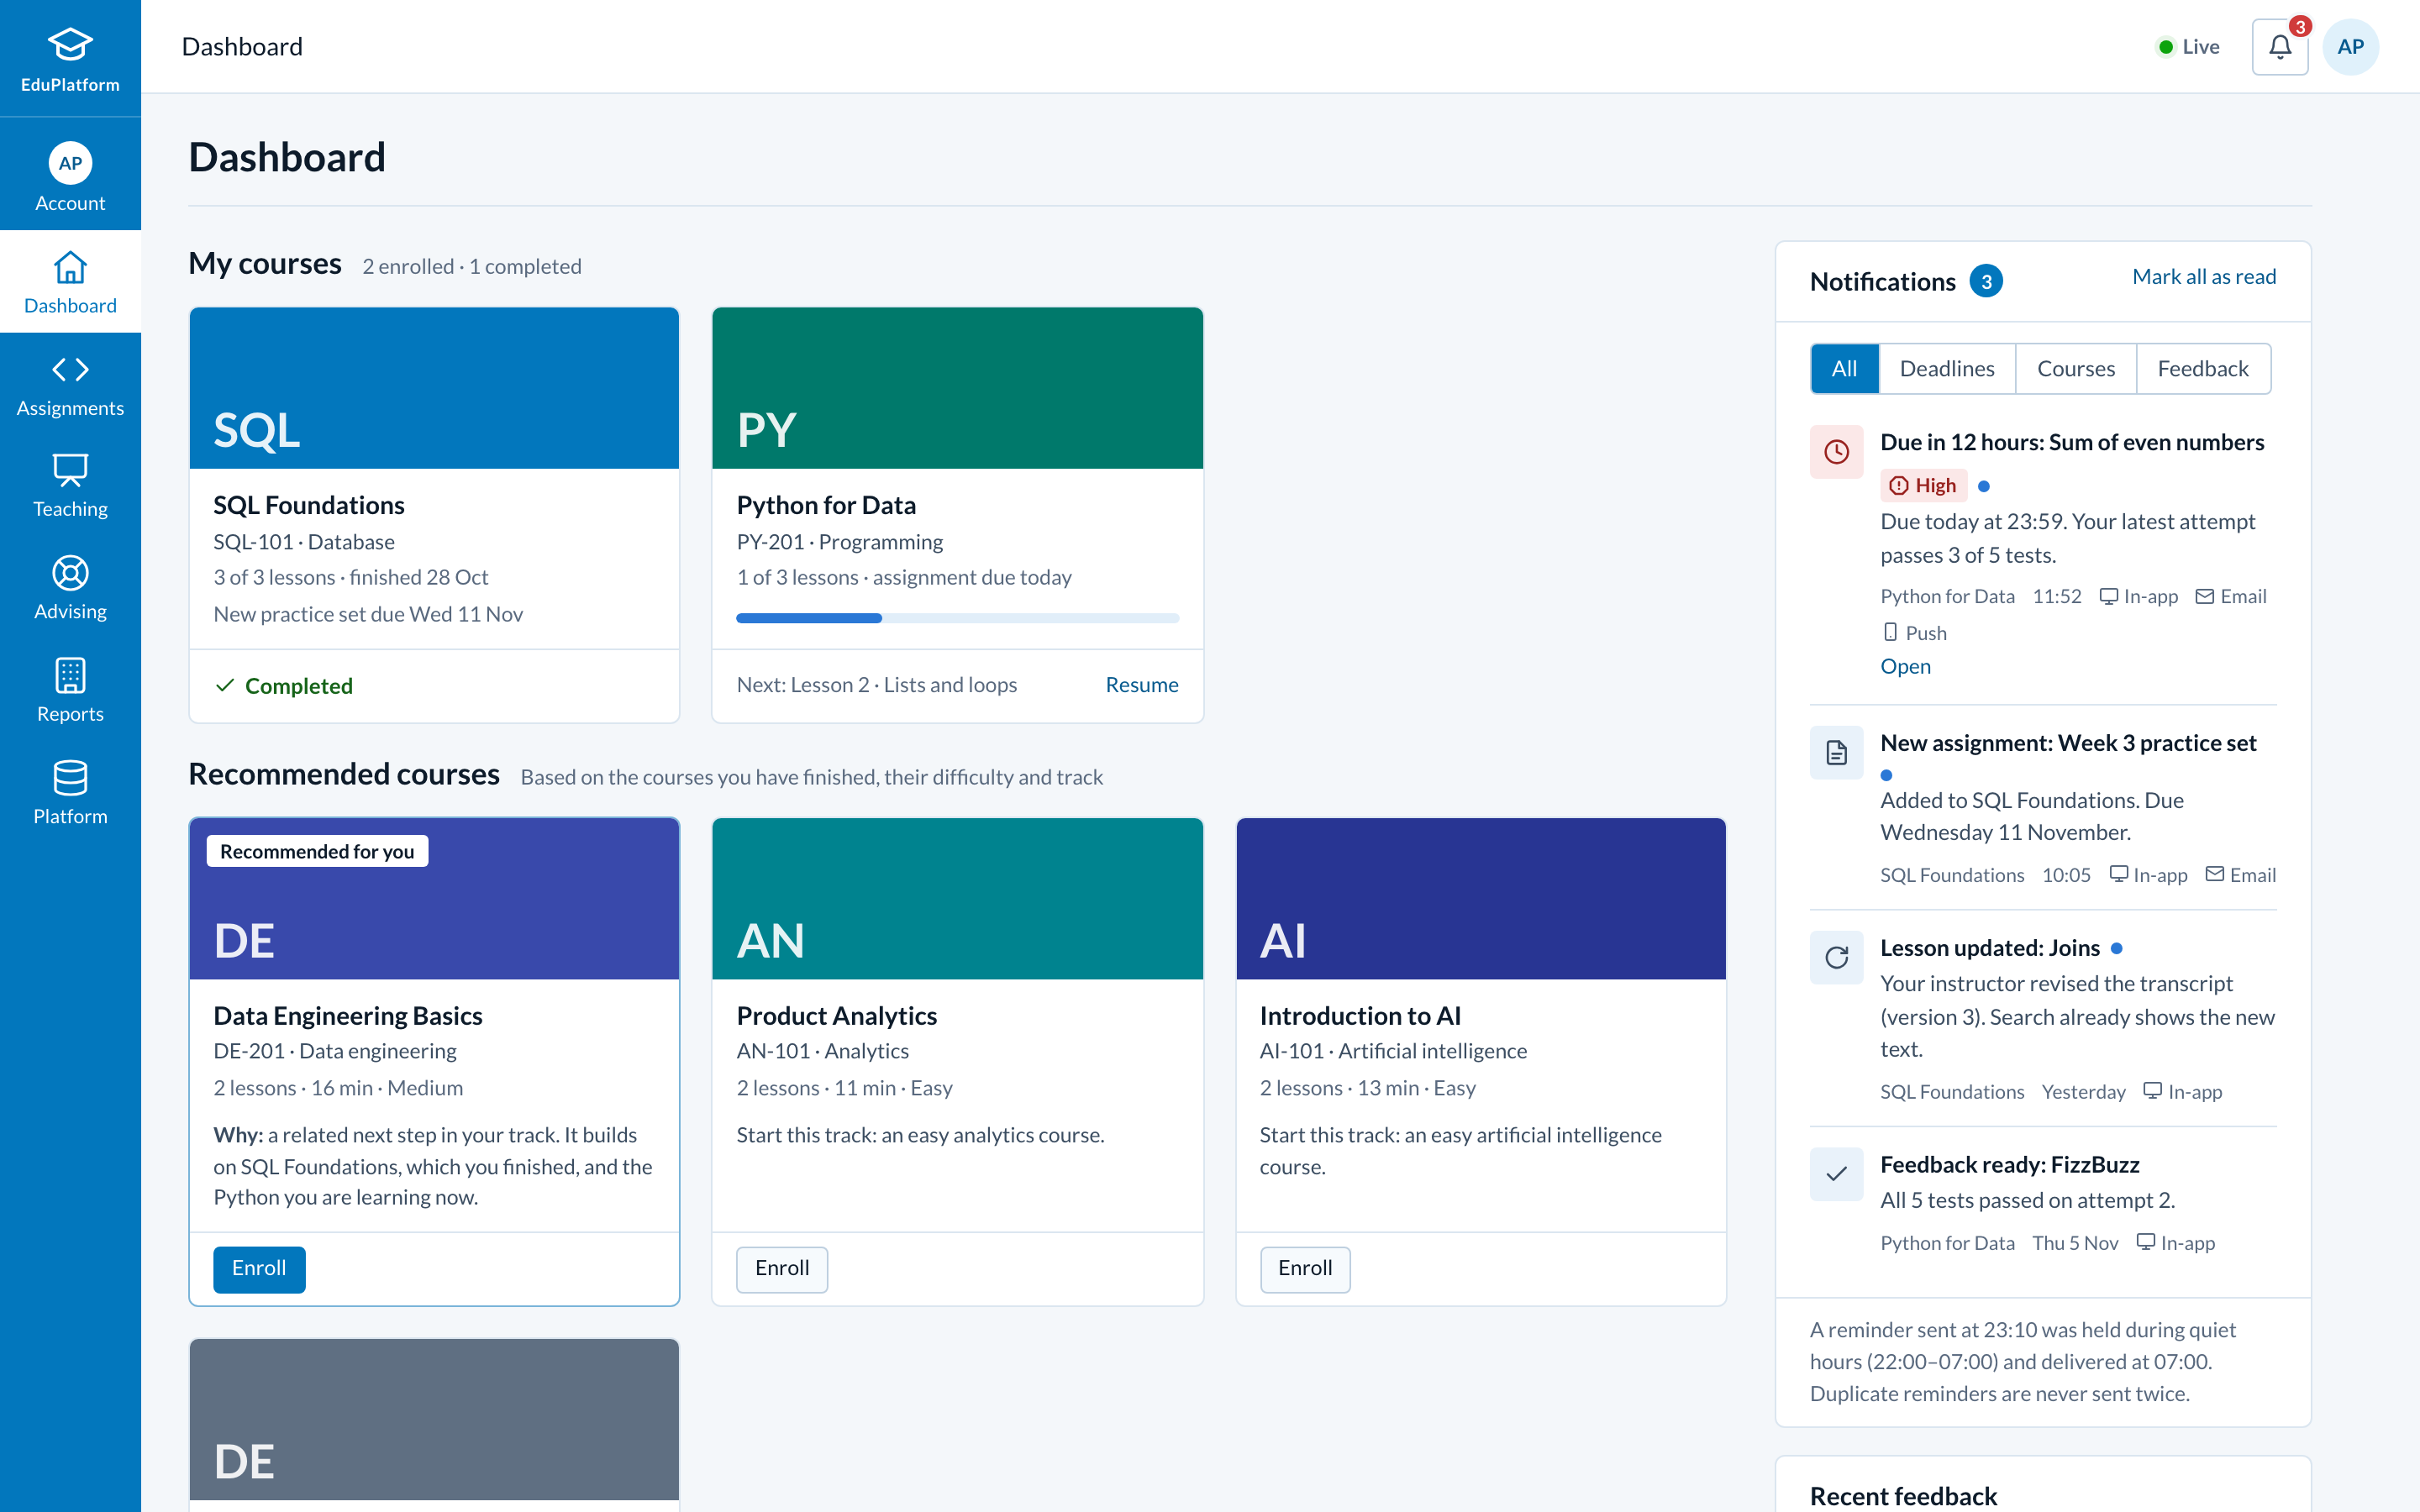
\includegraphics[width=\textwidth]{figures/mockup/learner-home.png}
\todofix{thay bằng screenshot mới (hoặc giữ mockup có chủ đích)}
\caption{Mockup: trang chủ người học với thông báo (BR1) và gợi ý khoá học kèm lý do (BR2)}
\label{fig:mock-learner}
\end{figure}

\subsection{Hệ thống thiết kế}

\begin{itemize}
  \item \textbf{Token thiết kế} cho màu, khoảng cách, bo góc và bóng đổ, có bộ giá trị riêng cho chế độ sáng và tối. Người dùng chuyển chế độ bằng một công tắc; mặc định theo hệ điều hành.
  \item \textbf{Bảng màu biểu đồ đã kiểm định}: màu phân loại theo thứ tự cố định và một dải màu xanh đơn sắc cho độ lớn (heatmap), đã kiểm tra khả năng phân biệt với người mù màu. Màu trạng thái (tốt, cảnh báo, nghiêm trọng, nguy hiểm) chỉ dùng cho trạng thái và luôn đi kèm biểu tượng và nhãn chữ, không bao giờ chỉ dựa vào màu.
  \item \textbf{Khả năng tiếp cận}: mọi biểu đồ có tooltip khi rê chuột và một bảng dữ liệu ``Xem dạng bảng'' thay thế; các nút có nhãn cho trình đọc màn hình; bố cục co giãn tới màn hình điện thoại mà không phải cuộn ngang.
  \item \textbf{Nhãn yêu cầu}: mỗi trang và mỗi khối được gắn nhãn BR tương ứng (có thể tắt). Nhãn này giúp truy vết từ giao diện về yêu cầu khi trình bày.
\end{itemize}

\subsection{Kiến trúc frontend}

Ứng dụng tổ chức theo \emph{không gian làm việc} (workspace), mỗi nhóm người dùng một workspace, chọn ở thanh bên (Bảng~\ref{tab:routes}). Thanh trên cùng có chỉ báo sự kiện trực tiếp (Server-Sent Events), thông báo của người học và trạng thái đăng nhập.

{\small
\begin{longtable}{@{}L{2.4cm}L{4.4cm}L{6.4cm}L{1.4cm}@{}}
\caption{Workspace, đường dẫn và trang}\label{tab:routes}\\
\toprule
\textbf{Workspace} & \textbf{Đường dẫn} & \textbf{Nội dung} & \textbf{BR} \\
\midrule
\endfirsthead
\toprule
\textbf{Workspace} & \textbf{Đường dẫn} & \textbf{Nội dung} & \textbf{BR} \\
\midrule
\endhead
Learner & \code{/learner} & Khoá học, gợi ý, phản hồi gần đây, thông báo & 1, 2 \\
Learner & \code{/learner/code-lab} & Trình soạn mã, phản hồi từng test, các lần nộp & 3 \\
Instructor & \code{/instructor/assessments} & Câu hỏi và chi tiết test case & 4 \\
Instructor & \code{/instructor/videos} & Heatmap theo phiên bản, lớp phủ hôm nay, thời điểm cần xem lại & 7 \\
Instructor & \code{/instructor/engagement} & Trung bình khoá học, học viên đang giảm & 8 \\
Instructor & \code{/instructor/content} & Xuất bản phiên bản, theo dõi đồng bộ, xem trước tìm kiếm & 8 \\
Advisor & \code{/advisor} & Hàng đợi rủi ro, phân rã điểm, lịch sử, cảnh báo & 5 \\
Org admin & \code{/admin} & Tiến độ tổ chức có ẩn nhóm nhỏ, xuất CSV & 6 \\
Data platform & \code{/pipeline} & Bộ đếm luồng, thông lượng, topic, DLQ, silver & -- \\
\bottomrule
\end{longtable}}

Các workspace Instructor, Advisor và Org admin được bảo vệ bằng một thẻ đăng nhập nhận token của vai trò. Token được giữ trong phiên của tab trình duyệt và dùng chung cho mọi trang của workspace. Máy chủ tự ánh xạ token sang danh tính, vai trò và phạm vi khoá học hoặc tổ chức; giao diện không tự khai báo quyền. Các điều khiển chỉ dành cho demo (giả lập sự kiện LMS, bộ sinh telemetry) được tách vào các khối ``Demo controls'' viền nét đứt. Biểu đồ được vẽ bằng SVG thuần với chiều rộng thật của phần tử, nên chữ không bị co giãn.

\subsection{Các màn hình chính}

Các ảnh trong mục này được chụp từ ứng dụng thật chạy trên dữ liệu của hệ thống (chế độ tối), trừ khi ghi là mockup.

\begin{figure}[H]
\centering
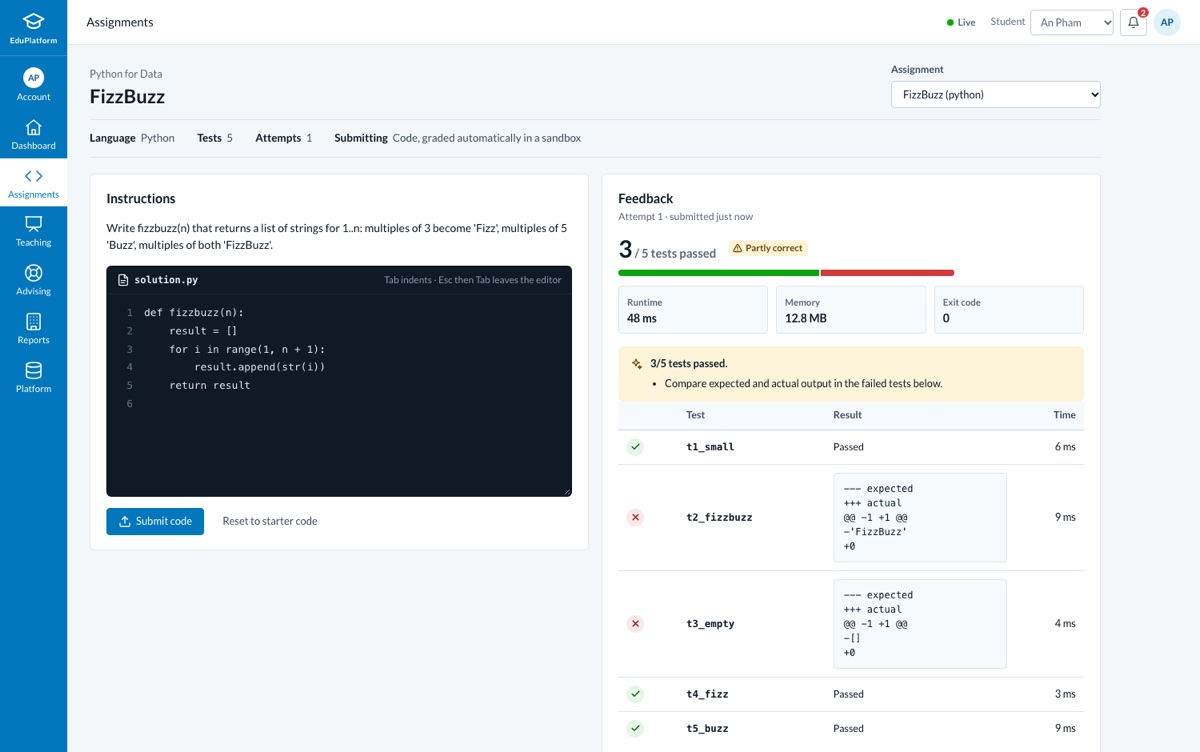
\includegraphics[width=\textwidth]{figures/ui/code-lab.jpg}
\todofix{chụp lại ảnh mới}
\caption{Code lab (BR3): bài nộp FizzBuzz được chấm trong sandbox, phản hồi từng test kèm diff}
\label{fig:ui-codelab}
\end{figure}

\begin{figure}[H]
\centering
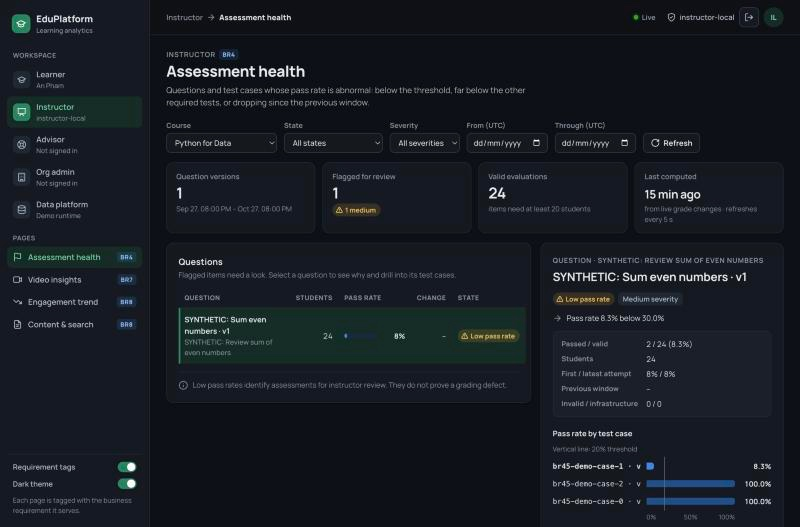
\includegraphics[width=\textwidth]{figures/ui/assessment-health.jpg}
\todofix{chụp lại ảnh mới}
\caption{Assessment health (BR4): câu hỏi bị gắn cờ và tỷ lệ đạt theo từng test case so với ngưỡng 20\%}
\label{fig:ui-br4}
\end{figure}

\begin{figure}[H]
\centering
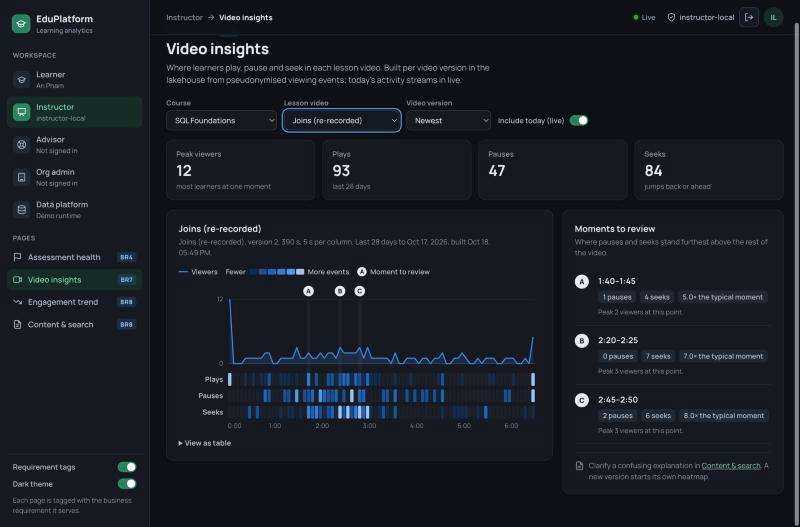
\includegraphics[width=\textwidth]{figures/ui/video-insights.jpg}
\todofix{chụp lại ảnh mới}
\caption{Video insights (BR7): heatmap play/pause/seek của phiên bản 2 video ``Joins'' (390 giây), kèm các thời điểm cần xem lại}
\label{fig:ui-br7}
\end{figure}

\begin{figure}[H]
\centering
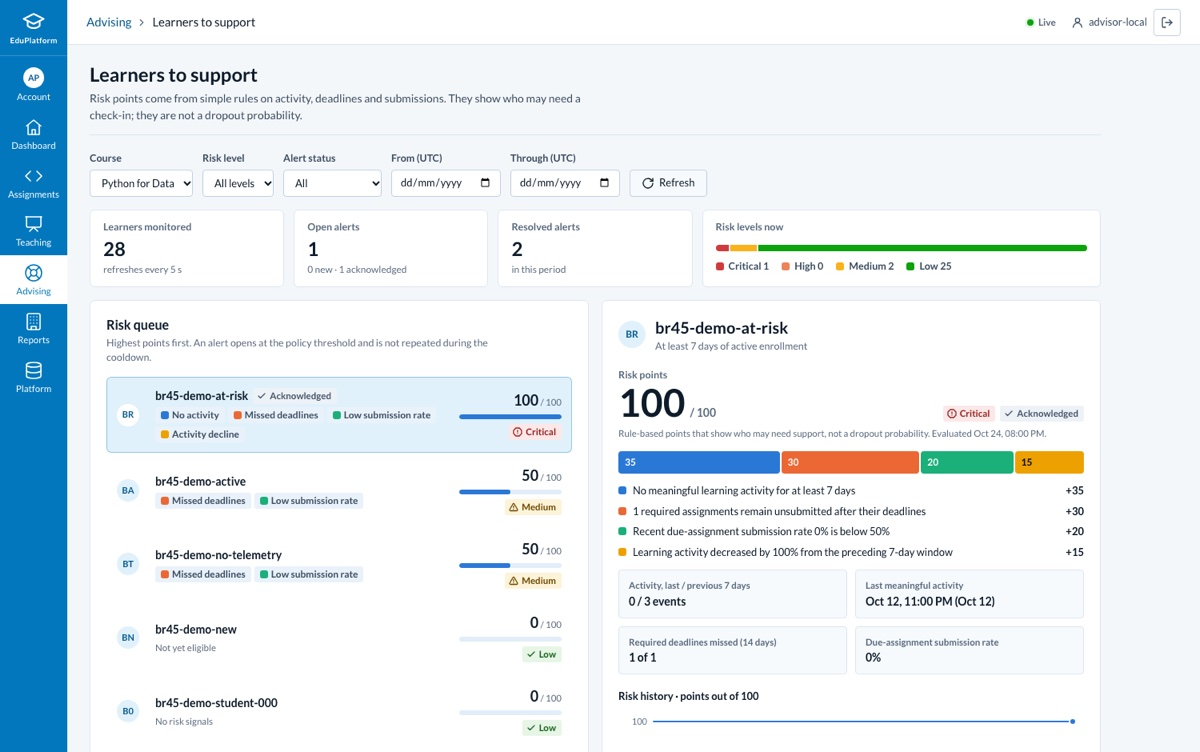
\includegraphics[width=\textwidth]{figures/ui/advisor.jpg}
\todofix{chụp lại ảnh mới}
\caption{Learners to support (BR5): hàng đợi rủi ro và phân rã 100 điểm thành 35 + 30 + 20 + 15}
\label{fig:ui-br5}
\end{figure}

\begin{figure}[H]
\centering
\begin{subfigure}{0.86\textwidth}
  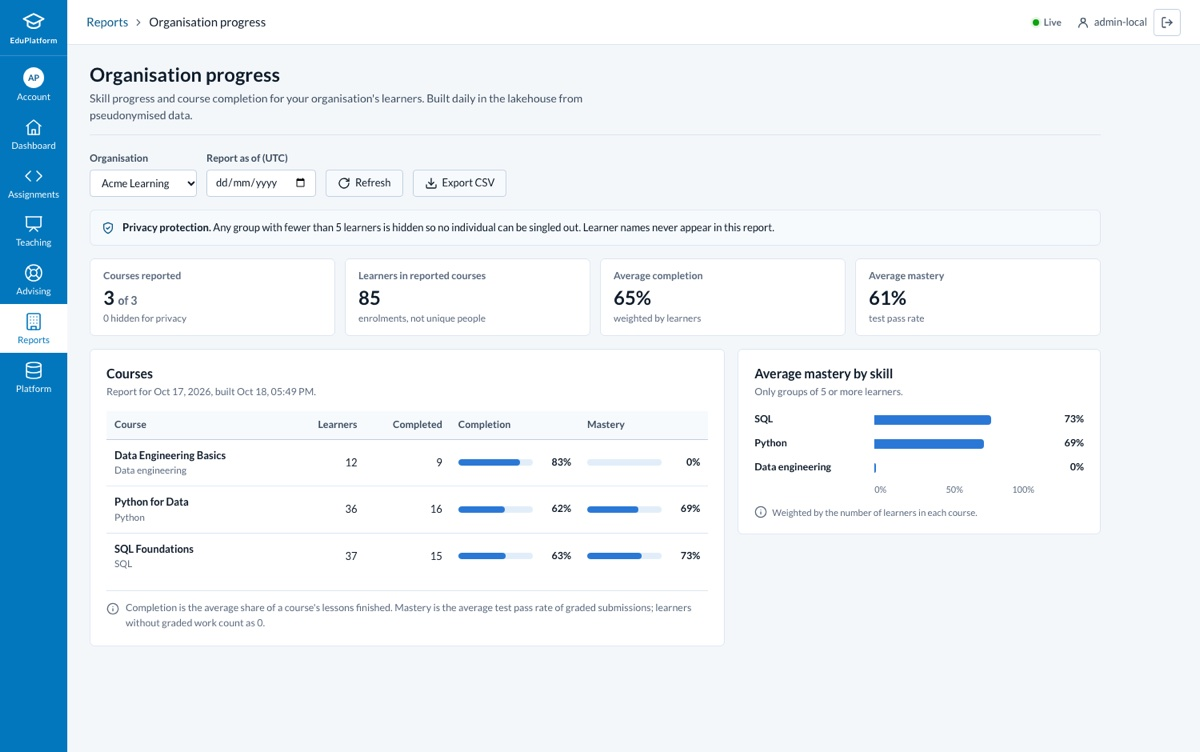
\includegraphics[width=\textwidth]{figures/ui/admin-acme.jpg}
\todofix{chụp lại ảnh mới}
  \caption{Acme Learning: mọi nhóm đủ 5 người nên được báo cáo}
\end{subfigure}\\[6pt]
\begin{subfigure}{0.86\textwidth}
  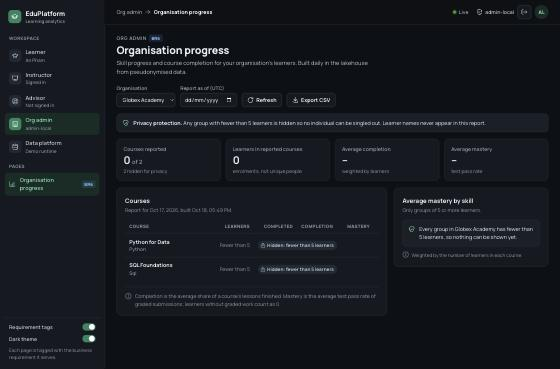
\includegraphics[width=\textwidth]{figures/ui/admin-globex.jpg}
\todofix{chụp lại ảnh mới}
  \caption{Globex Academy: mọi nhóm dưới 5 người nên bị ẩn, không lộ tỷ lệ hay quy mô chính xác}
\end{subfigure}
\caption{Organisation progress (BR6): k-anonymity với $k = 5$}
\label{fig:ui-br6}
\end{figure}

\begin{figure}[H]
\centering
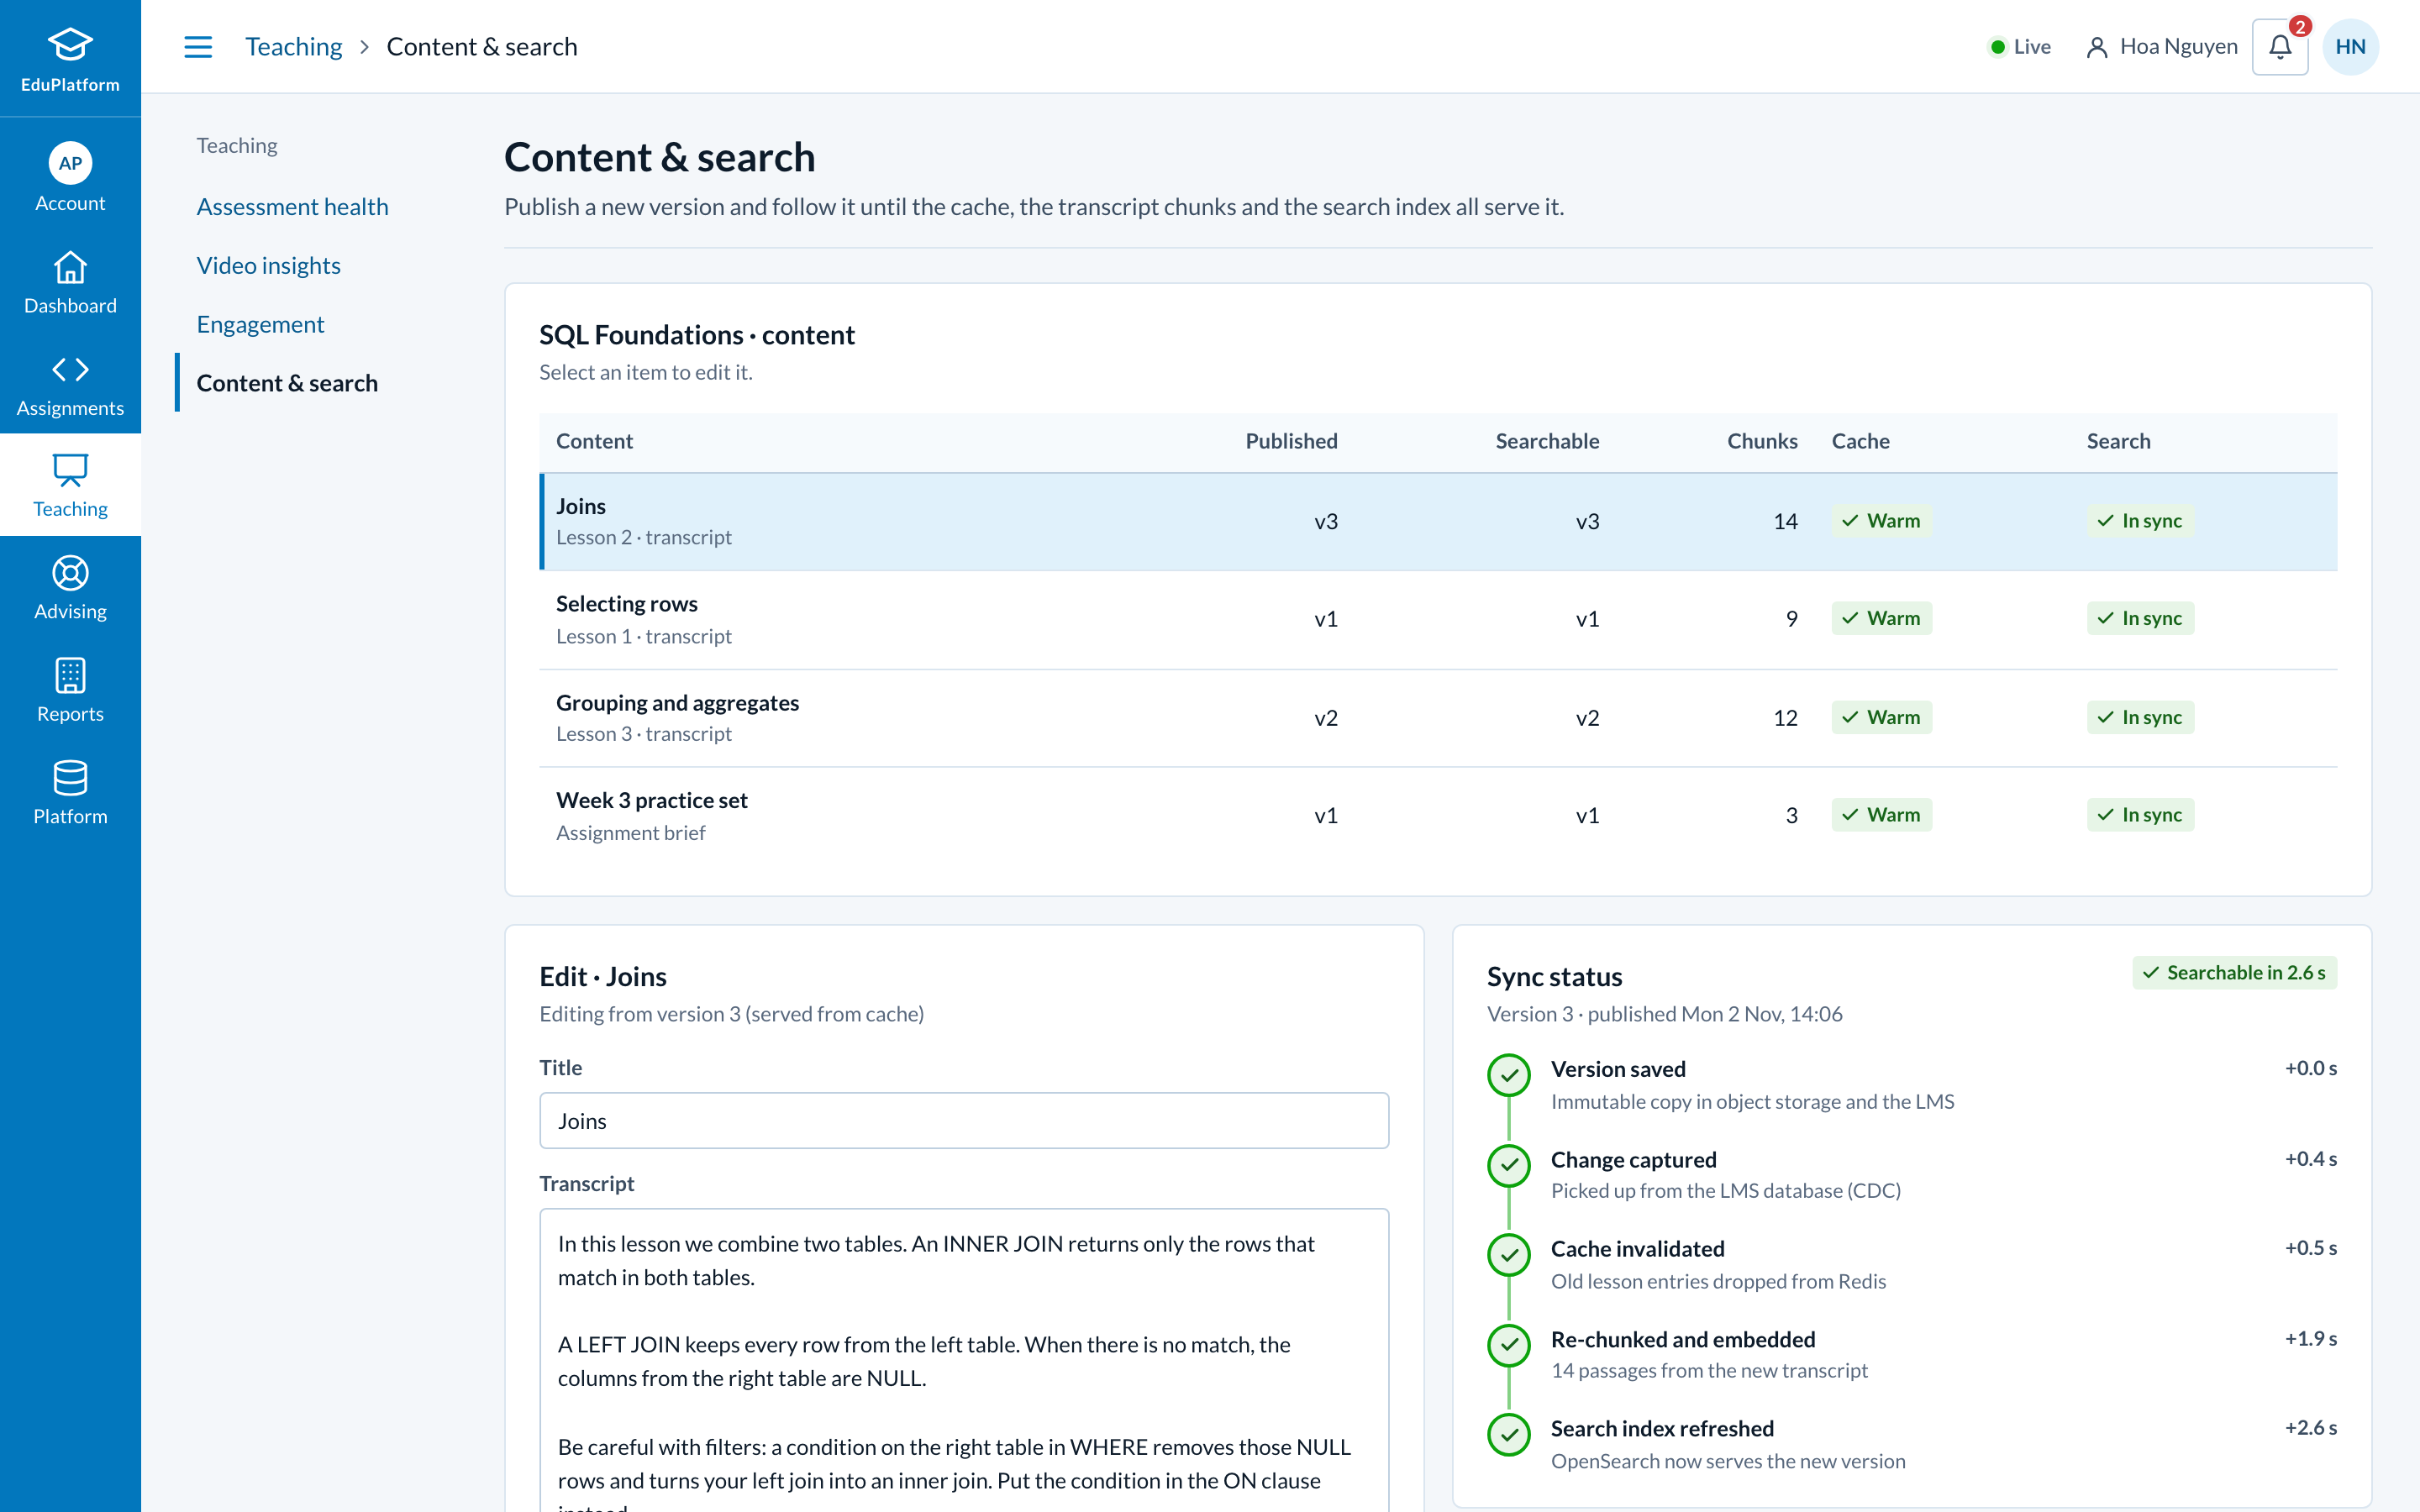
\includegraphics[width=\textwidth]{figures/mockup/instructor-content.png}
\todofix{thay bằng screenshot mới (hoặc giữ mockup có chủ đích)}
\caption{Mockup: Content \& search (BR8), theo dõi một phiên bản từ khi xuất bản đến khi tìm kiếm được}
\label{fig:mock-br8}
\end{figure}

\begin{figure}[H]
\centering
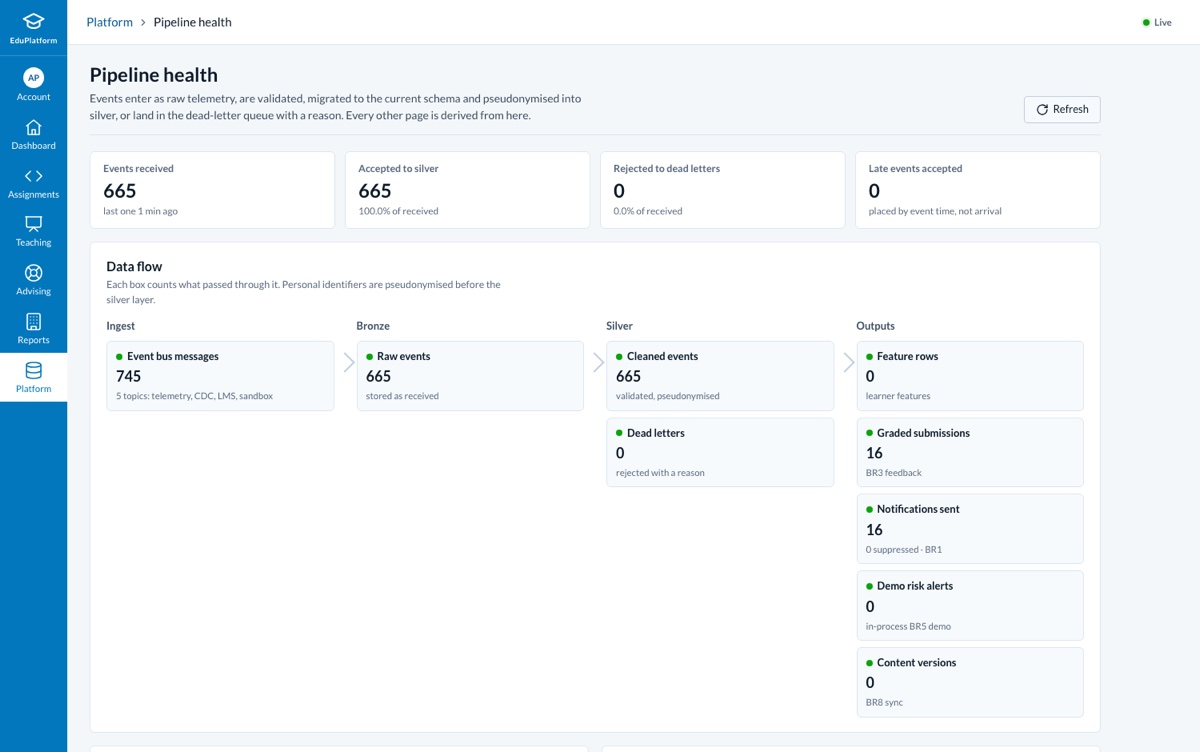
\includegraphics[width=\textwidth]{figures/ui/pipeline.jpg}
\todofix{chụp lại ảnh mới}
\caption{Pipeline health (chế độ sáng): bộ đếm của từng chặng trong luồng dữ liệu}
\label{fig:ui-pipeline}
\end{figure}

\begin{figure}[H]
\centering
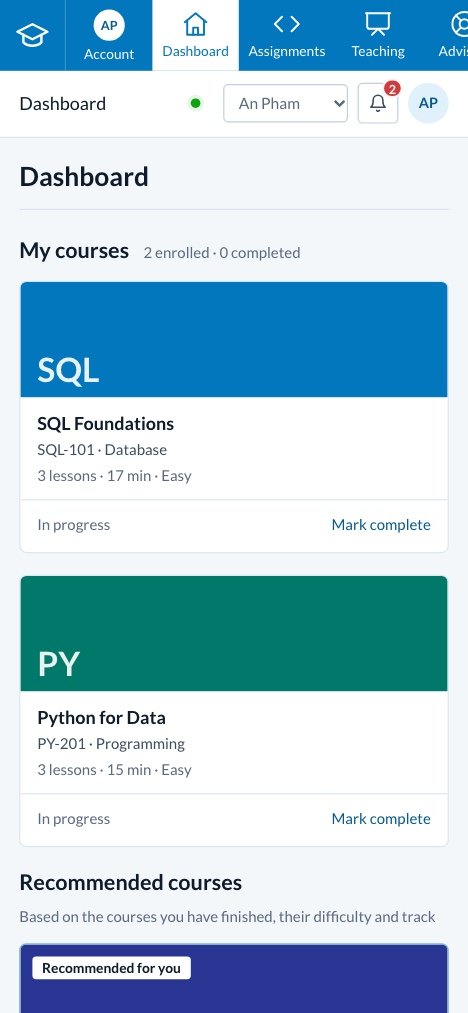
\includegraphics[width=0.42\textwidth]{figures/ui/learner-mobile.jpg}
\todofix{chụp lại ảnh mới}
\caption{Trang người học trên màn hình điện thoại (390 px): thanh bên chuyển thành tab ngang}
\label{fig:ui-mobile}
\end{figure}

\subsection{Kiểm thử giao diện}

Giao diện được kiểm chứng bằng ba cách:
\begin{itemize}
  \item \textbf{Biên dịch kiểu nghiêm ngặt}: TypeScript ở chế độ \code{strict}; bản build production thành công.
  \item \textbf{Kiểm tra thủ công trên trình duyệt} với dữ liệu thật ở chế độ sáng, tối, desktop và điện thoại. Một bài nộp thật đi qua sandbox và sinh ra một thông báo mới; các trang BR6--BR8 đọc mart thật từ Trino.
  \item \textbf{Kiểm thử chấp nhận bằng Playwright} (\code{apps/web/tests}), được cập nhật cho cấu trúc trang mới với các khẳng định nghiệp vụ giữ nguyên. Lần chạy sau khi thiết kế lại cho kết quả: ba test đạt (thông tin đăng nhập sai bị từ chối; báo cáo tổ chức ẩn nhóm nhỏ và chặn truy cập ngoài phạm vi; heatmap theo phiên bản và xu hướng tương tác). Các test còn lại cần những dịch vụ không chạy vào thời điểm đó (container \code{br45}, OpenSearch, lớp phủ trực tiếp) nên chưa được chạy lại trên giao diện mới.
\end{itemize}